\documentclass{beamer}

\usepackage[T2A]{fontenc}
\usepackage[utf8]{inputenc}
\usepackage[russian]{babel}
\usepackage{biblatex}
\usepackage{csquotes}
\bibliography{doc/doc.bib}

\usepackage{graphicx}
\graphicspath{ {./assets/} }

\usetheme{Madrid}

\title{How to Write Formal e-mails in English}
\author{Sherstobitov Andrei}
\date{April 2024}

\begin{document}

\begin{frame}
  \titlepage
\end{frame}

\begin{frame}{Today we'll discuss:}
  \begin{enumerate}
    \item Rules of formal e-mail writing described by ConsultantPlus.
    \item Additional rules in various universities of United Kingdom.
  \end{enumerate}
\end{frame}

\begin{frame}{ConsultantPlus \cite{ConsultantPlus} suggests}
  \begin{enumerate}
    \item Write the subject of the letter.
    \item Address recipient by name.
    \item Write briefly, straight to the point.
    \item Name the attached files clearly.
    \item Sign the letter.
    \item Reread the letter before sending.
  \end{enumerate}
\end{frame}

\begin{frame}{Write the subject of the letter.}
  \begin{itemize}
    \item Keep the subject straight to the point.
    \item Do not use spam words.
  \end{itemize}

  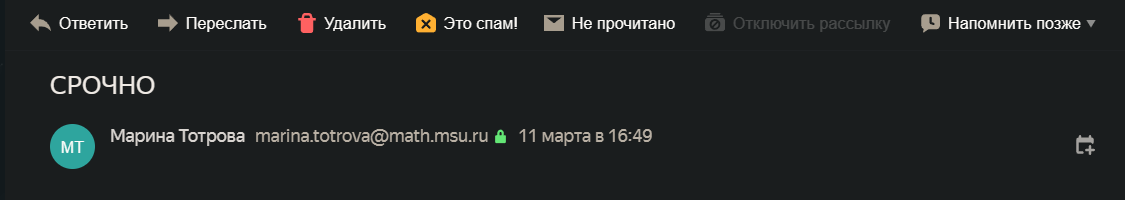
\includegraphics[width=\linewidth]{theme-bad.png}

  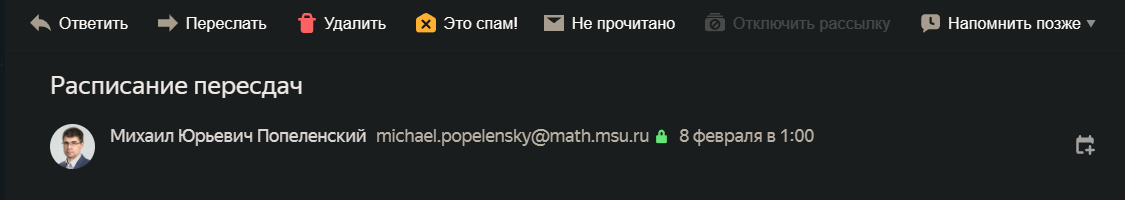
\includegraphics[width=\linewidth]{theme-good.png}

\end{frame}


\begin{frame}{Address recipient by name.}
  \begin{itemize}
    \item It is polite and it will keep the letter from spam folder.
    \item Greeting -- the only place to use exclamation point in formal letter.
  \end{itemize}
  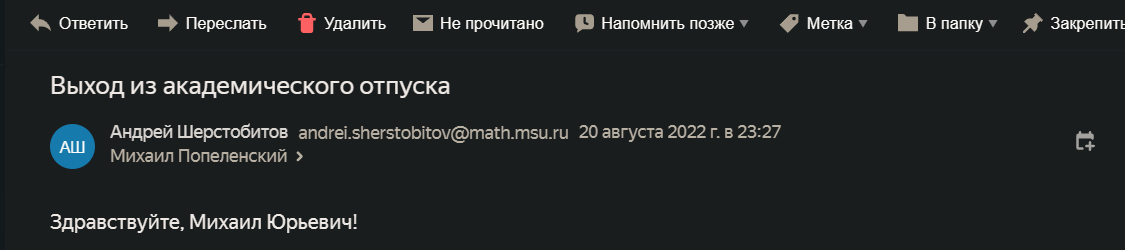
\includegraphics[width=\linewidth]{greeting.png}
  \begin{itemize}
    \item If it not the first letter during the day, you can do the next:
  \end{itemize}
  \begin{center}
    \begin{tabular}{ |c|l c c| }
      \hline
      Subject & Re: Семинар 02.05.2024    & \quad & \quad \\
      \hline
              & \begin{tabular}{@{}l}
        Геннадий Иванович, \\
        не смогу прийти, сломал ногу.
      \end{tabular} & \quad & \quad \\
    \end{tabular}
  \end{center}
\end{frame}

\begin{frame}{Write briefly, straight to the point.}
  \begin{itemize}
    \item State the main theme of the letter in the first lines.
    \item In the following paragraphs provide arguments and explanations.
    \item Clearly formulate questions and requests.
    \item Indicate the desired response time.
  \end{itemize}

  \begin{center}
    \begin{tabular}{ |l c c| }
      \hline
      Спецсеминар               & \quad & \quad \\
      \hline
      \begin{tabular}{@{}l@{}}
        Всем добрый день!                                      \\
        Начинаем проводить еженедельные встречи (спецсеминар)  \\
        по вторникам, 16:45 во 2 корпусе. Пока не определилась \\
        аудитория, собираемся около кафедральной комнаты.      \\
        Прошу о неявке предупредить заранее (до вторника).
      \end{tabular} & \quad & \quad \\
    \end{tabular}
  \end{center}
\end{frame}

\begin{frame}{Name the attached files clearly.}
  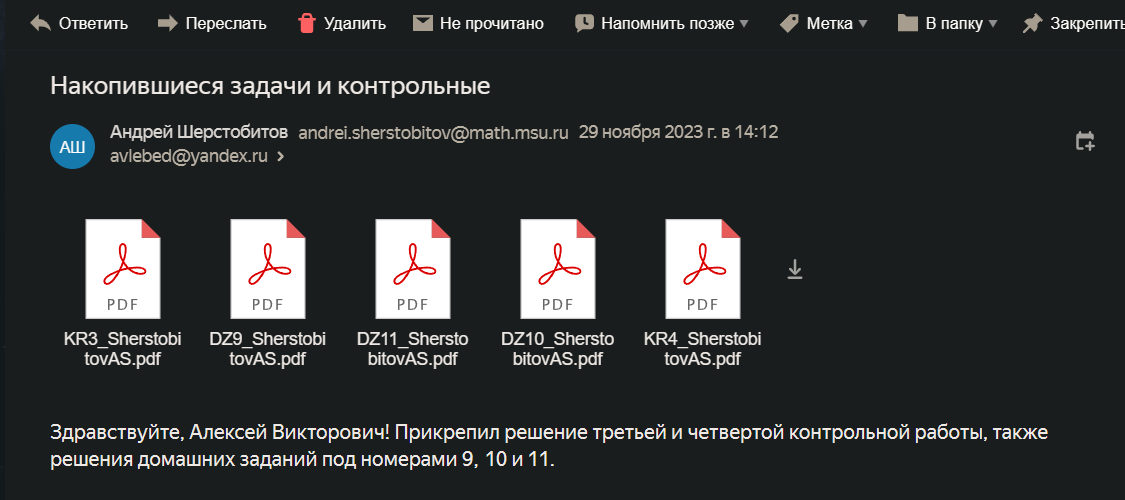
\includegraphics[width=\linewidth]{attached.png}
\end{frame}

\begin{frame}{Sign the letter.}
  \begin{itemize}
    \item Write your first and last name.
    \item Depending on the situation, you can add status or position.
  \end{itemize}

  \begin{center}
    \begin{tabular}{ |l|l| }
      \begin{tabular}{l}
        С уважением,       \\
        Шерстобитов Андрей \\
        Студент 531 учебной группы
      \end{tabular} & \begin{tabular}{l}
        С уважением,       \\
        Шерстобитов Андрей \\
        Разработчик сетевого отдела
      \end{tabular} \\
    \end{tabular}
  \end{center}
\end{frame}

\begin{frame}{Reread and send the letter.}
  \begin{itemize}
    \item Reread the text, correct typos and errors.
    \item Check that intended files are attached.
    \item Send the letter in work time.
  \end{itemize}
\end{frame}

\begin{frame}{Leeds Beckett University \cite{Beckett} suggests}
  \begin{enumerate}
    \item E-mail is not always the best form of communication.
    \item Make the title relevant.
    \item Do not ignore basic English.
    \item Keep it short.
    \item Be careful about replying to all.
  \end{enumerate}
\end{frame}

\begin{frame}{E-mail is not always the best form of communication.}
  \begin{itemize}
    \item Before sending an e-mail, consider whether it is the best way to communicate.
    \item Do not discuss urgent issues via e-mail.
    \item Don't say anything you wouldn't say in person.
  \end{itemize}
\end{frame}

\begin{frame}{Do not ignore basic English. Be careful about replying to all.}
  \begin{itemize}
    \item Do not completely ignore the basic use of grammar and spelling.
    \item Do not rush with the answer, wait until you have time to respond properly.
    \item Limit the number of recipients to whom you send a message to those who need to
          know about it.
  \end{itemize}

  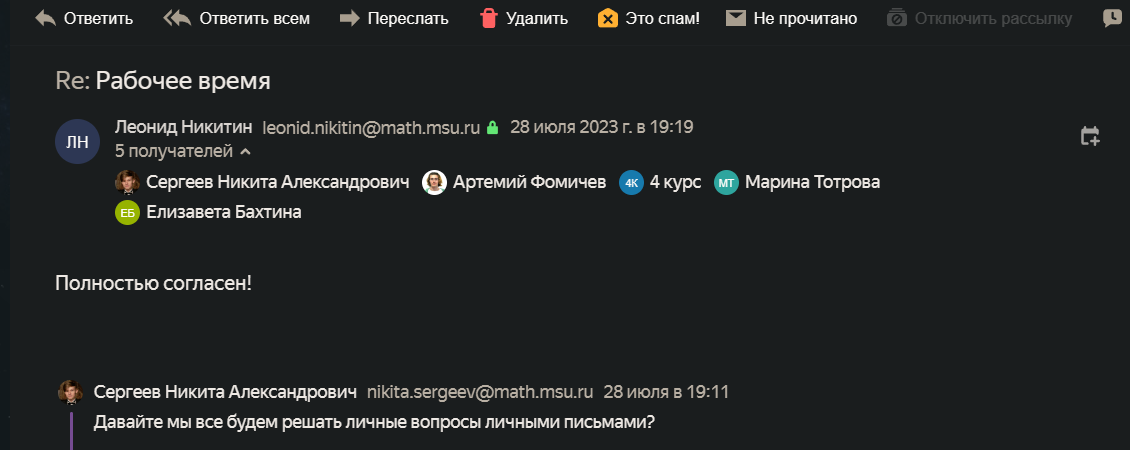
\includegraphics[width=\linewidth]{reply-to-all.png}

\end{frame}

\begin{frame}{University of Bolton \cite{Bolton} legal considerations}
  \begin{displayquote}
    Email is a risky communications channel for sharing private or confidential
    information for a number of reasons:

    Individuals (staff, students, anyone) have a right to see \textbf{any information that is written about them} in
    an email whether University or personal email. They can request disclosure via a Subject Access
    Request to the University.
  \end{displayquote}
\end{frame}

\begin{frame}{University of Bolton distinguishing suggestions}
  \begin{itemize}
    \item WRITING IN CAPITAL LETTERS IN AN EMAIL IS CONSIDERED THE EQUIVALENT OF
          SHOUTING AND BEING AGGRESSIVE. Avoid.
    \item Be careful when including a long email trail in a reply or forward; they can increase the risks of some
          recipients receiving information that was not intended for them.
    \item Always make sure that any file attachment you are sending, that contains anyone's personal data, is
          encrypted.
    \item Do not say anything that might discredit the University or anything which might imply a legal
          obligation.
  \end{itemize}
\end{frame}

\begin{frame}{University of Liverpool \cite{Liverpool} about attachments.}
  \begin{itemize}
    \item Be very careful when opening attachments.
    \item Be selective in the sending of attachments, use shared drives instead.
    \item Consider the file format of the attachment.
    \item Be careful about the size of an attachment.
    \item Use a virus scanner.
  \end{itemize}
\end{frame}

\begin{frame}{University of Sussex \cite{Sussex} first bullet in the guidance.}
  \begin{displayquote}
    First: think before you send an email. Is it the best way to communicate? A more complex
    message might be better discussed face to face or delivered as a presentation
  \end{displayquote}
\end{frame}

\begin{frame}{Wall Street English \cite{WallStreet} formats of formal email.}
  \begin{enumerate}
    \item Introduction. Any e-mail should start with the greeting.
          \begin{itemize}
            \item Dear Mr/Mrs/Ms (surname of the recipient, e.g. Mr Black)
            \item Dear Sir/Madam (if you don't know the name of the recipient)
          \end{itemize}
    \item Introductory sentence that indicates clearly the reason for writing.
          \begin{itemize}
            \item I am writing with regard to...
            \item I am writing in connection with...
            \item I am writing in reference to...
          \end{itemize}
    \item If you're writing an email to send information, you can start with:
          \begin{itemize}
            \item I am writing to let you know...
            \item I am delighted to tell you...
            \item I regret to inform you that...
          \end{itemize}
    \item If you're replying to an email you received, you can say:
          \begin{itemize}
            \item I am writing in response to...
            \item I am writing in reply to...
            \item I am writing to thank you for...
          \end{itemize}
  \end{enumerate}
\end{frame}

\begin{frame}{Wall Street English formats of formal email.}
  \begin{enumerate}
    \setcounter{enumi}{4}
    \item Body of the text.
          \begin{itemize}
            \item It's useful to prepare an initial draft and then proceed with any corrections.
            \item The text should be divided into short paragraphs.
          \end{itemize}
    \item There are various ways to write a final invitation before ending the email, such as:
          \begin{itemize}
            \item I look forward to hearing from you soon
            \item Thank you in advance
            \item For further information, please do not hesitate to contact me
            \item Please let me know if you have any questions
            \item Thanks for your attention
          \end{itemize}
    \item Conclusion. The most common way to end an email are:
          \begin{itemize}
            \item Best/Kind regards...
            \item Yours faithfully (if you began with "Dear Sir/Madam" because you don't know the name of the recipient)
            \item Yours sincerely (if you began with "Dear Mr/Mrs/Ms + surname")
          \end{itemize}
  \end{enumerate}
\end{frame}

\begin{frame}{Examples of formal emails in English.}
  \begin{center}
    \begin{tabular}{ |c|l| }
      \hline
      Subject & Exciting discovery conserning the harmony series \\
      \hline  & \begin{tabular}{@{}l@{}}
        Dear Viktor Antonovich,                                  \\
        \\
        I hope this letter finds you well. I am writing to share \\
        with you an exciting discovery I have made regarding the \\
        sum of the harmonic series. After thorough research      \\
        and analysis, I have successfully derived a formula      \\
        that accurately calculates this sum.                     \\
        I would be grateful if you could review my findings and  \\
        provide any feedback or suggestions for improvement.     \\
        Please feel free to contact me at your convenience       \\
        to discuss this further.                                 \\
        \\
        Yours sincerely, Sherstobitov Andrei.
      \end{tabular}
    \end{tabular}
  \end{center}
\end{frame}

\begin{frame}{Examples of formal emails in English.}
  \begin{center}
    \begin{tabular}{ |c|l| }
      \hline
      Subject & Re: Exciting discovery conserning the harmony series \\
      \hline  & \begin{tabular}{@{}l@{}}
        Dear Andrei,                                                     \\
        I trust this letter reaches you in good spirits. I have received \\
        your letter regarding your supposed "exciting discovery"\        \\
        concerning the sum of the harmonic series. While I commend       \\
        your enthusiasm for mathematical exploration, I must express     \\
        my reservations about the validity of your findings.             \\
        Upon initial review, it appears that your derivation overlooks   \\
        fundamental principles of calculus. I would strongly advise you  \\
        to revisit the fundamental concepts covered in our lectures.
        \\
        I am open to discussing your work further, but I urge you to     \\
        reconsider your approach and ensure that your future             \\
        endeavors are grounded in sound mathematical reasoning.          \\
        Yours sincerely, Victor Antonovich.
      \end{tabular}
    \end{tabular}
  \end{center}
\end{frame}

\begin{frame}
  \printbibliography
\end{frame}

\begin{frame}
  \centering \Huge
  Thank you for attention!
\end{frame}

\end{document}
